
In the following, we will summarise the results obtained for the IPAC
data set. We deal with the different physical parameters in separate
Sections. We start by reporting the cross validation Root Mean Square
Errors (RMSE) and Root Median Square Error (RMDSE ) for the five-fold
cross-validation strategy, and we subsequently discuss the accuracy of
the predictions with respect to literature values where available.

\subsubsection{Effective temperature models}

Table \ref{tab:model_TSD_IPAC} summarises the RMSE/RMDSE for the
complete set of models: the minimum $\chi^2$ estimate based on the
full spectrum ($\chi^2$), the projection pursuit regression based on
the ICA components (PPR-ICA) and some models trained on the spectral
features proposed by the GA (GA-RF, GA-GBM, GA-SVR, GA-NNET, GA-MARS,
GA-KPLS). For each model, we report the RMSE/RMDSE obtained for
several noise levels of the training sets.

% According to Joaqu. this is with respect to the spectral types
% 
\begin{table*}\centering
\ra{1.3}
\begin{tabular}{@{}rrrcrrcrr@{}}\toprule
& \multicolumn{2}{c}{$SNR = 10$} & \phantom{ab}& \multicolumn{2}{c}{$SNR = 50$} &
\phantom{ab} & \multicolumn{2}{c}{$SNR = \infty$}\\
\cmidrule{2-3} \cmidrule{5-6} \cmidrule{8-9}
$Regression Models$ & $RMSE$ & $RMDSE$ && $RMSE$ & $RMDSE$ && $RMSE$ & $RMDSE$ \\ \midrule
$\chi^2$    & {\bf 147} & 79       && {\bf 121} & {\bf 56}  && {\bf 126} & {\bf 57} \\
$ PPR-ICA$  & 188       & 126      && 164       & 95        && 191       & 130 \\
GA-RF       & 160       & 97       && 196       & 103       && 145       & 94 \\
GA-GBM      & 175       & 105      && 225       & 99        && 185       & 94 \\
GA-SVR      & 203       & 112      && 285       & 106       && 368       & 154 \\
GA-NNET     & 221       & 84       && 313       & 111       && 395       & 202 \\
GA-KNN      & 183       & 119      && 193       & 109       && 224       & 110  \\
GA-MARS     & 222       & 76       && 361       & 103       && 374       & 157 \\
GA-KPLS     & 227       & {\bf 72} && 331       & 123       && 409       & 208 \\
\bottomrule
\end{tabular}
\caption {RMSE and RMDSE for the various regression models that predict $T_{eff}$ (K).} 
\label{tab:model_TSD_IPAC} 
% \end{center}
\end{table*}

Again, as in the IRTF case, we see that the compression of the spectra
results in a performance degradation. Figure \ref{} 

\begin {figure*}
 \centering
  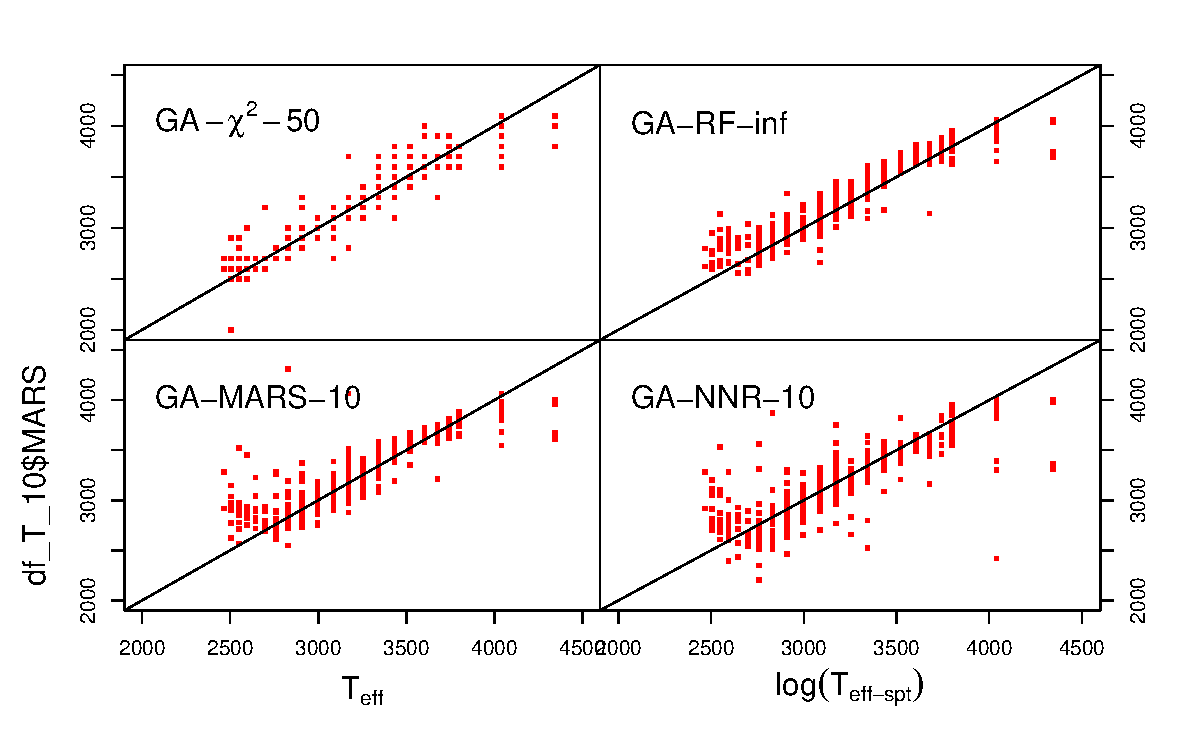
\includegraphics[width=11cm]{figs/ipac-teff.pdf}
  \caption{Comparison between Temperature estimations from Theoretical Temperature 
  in x axis and the modeled ICA based estimation at SNR=$\infty$ on y-axis}
 \label{fig:ipac_teff}
\end {figure*}



%%%%%%%%%%%%%%%%%%%%%%%%%%%%%%%%%%%%%%%%%%%%%%%%%%%%%%%%%%%%%%%
% Comparison with the Teff from SpType calibration.
%%%%%%%%%%%%%%%%%%%%%%%%%%%%%%%%%%%%%%%%%%%%%%%%%%%%%%%%%%%%%%%

{\bf Explain the spt-teff calibration used.}

{\bf Biases?}

{\bf We do have problems with the prediction at low temperatures when
trained with SNR= 10 or 50.}

{\bf Include plot with 4 models}


%%%%%%%%%%%%%%%%%%%%%%%%%%%%%%%%%%%%%%%%%%%%%%%%%%%%%%%%%%%%%%%
% Comparison with predictions from Cesetti's features. 
%%%%%%%%%%%%%%%%%%%%%%%%%%%%%%%%%%%%%%%%%%%%%%%%%%%%%%%%%%%%%%%

Having shown that the feature selection with GAs degrades the
performance of regression models, one can wonder whether a different
feature selection procedure would produce better results. In
particular, we investigate the possibility that the features proposed
by \cite{cesetti} result in a performance equal to or even better than
the one achieved with $\chi^2$.

%\begin{table}
%\begin{center}
%\begin{tabular}{rrrr}
%  \hline
%  $\lambda_1$ & $\lambda_2$ & $\lambda_{cont;1}$ & $\lambda_{cont;2} $ \\ 
%  \hline
%8461 & 8474 & 8474 & 8484 \\
%8484 & 8513 & 8474 & 8484 \\
%8522 &  8562 & 8474 & 8484 \\
%8577 & 8619 & 8563 & 8577 \\
%8642 & 8682 & 8619 & 8642 \\
%8730 & 8772 & 8700 & 8725 \\
%8802 & 8811 & 8776 & 8792 \\
%8850 & 8890 & 8815 & 8850 \\
%9000 & 9030 & 8983 & 8998 \\
%9080  & 9100 & 9040 & 9050 \\
%\hline
%\end{tabular}
%\caption {Features selected by following suggestions from Cesetti et al, table 1. } 
%\label{tab:tab_CS_T}
%\end{center}
%\end{table}

We train the same regression models applied to the GA selected
features, to the features selected in \cite{cesetti}, again learning
from BT-Settl spectra of various SNRs and predicting over the IPAC
set. A summary of the results can be found in Table
\ref{tab:tab_CS_Model}, where we use CS- to indicate that the model was
trained using the features by \cite{cesetti}.

\begin{table*}
\begin{center}
\begin{tabular}{@{}rrrcrrcrr@{}}\toprule
& \multicolumn{2}{c}{$SNR = 10$} & \phantom{ab}& \multicolumn{2}{c}{$SNR = 50$} &
\phantom{ab} & \multicolumn{2}{c}{$SNR = \infty$}\\
\cmidrule{2-3} \cmidrule{5-6} \cmidrule{8-9}
$Regression Models$ & $RMSE$ & $RMDSE$ && $RMSE$ & $RMDSE$     && $RMSE$       & $RMDSE$ \\ \midrule
CS-RF   & 203       & 140       && 243       & {\bf 121} &&  {\bf 306} &  {\bf 172}  \\
CS-GBM  & {\bf 188} & {\bf 120} && {\bf 161} & 138       &&  337       &  222  \\
CS-SVR  & 197       & 135       && 379       & 194       &&  840       &  688  \\
CS-NNET & 207       & 135       && 514       & 296       &&  719       &  489  \\
CS-MARS & 252       & 124       && 789       & 186       && 3464       &  784  \\
CS-KNN  & 235       & 158       && 246       & 137       &&  314       &  175  \\
CS-KPLS & 250       & 201       && 741       & 361       && 2247       & 1424  \\
CS-RR   & 211       & 128       && 400       & 239       &&  828       &  774  \\

\hline
\end{tabular}
\caption {Performances of regression models trained on the features
  selected by \cite{cesetti} applied to BT-Settl spectra.}
\label{tab:tab_CS_Model}
\end{center}
\end{table*}

For SNR=10, the GA best models (GA-KPLS in RMDSE or GA-RF in RMSE)
outperform the best CS model (GA-GBM). For SNR=50 the situation
depends on the figure-of-merit used to compare the classifiers: in
RMSE the best model is CS-GBM while in RMDSE GA-GBM outperforms all
CS-models. Finally, for the unrealistic case of noiseless spectra,
Table \ref{tab:tab_CS_Model} shows an overwhelming degradation of the
prediction accuracy from CS- features. {\bf Overfitting?} But even in
the only case where the CS features outperform those selected by the
GA, the performance is below the one achieved by the minimum-$\chi^2$
approach.

%%% HERE 1 %%%

The relationship between the GA predicted Temperature and the one
measured by Rojas-Ayala can be found in the
Figure~\ref{fig:ipac_lt_lt}
\begin{figure}
 \begin{center}
 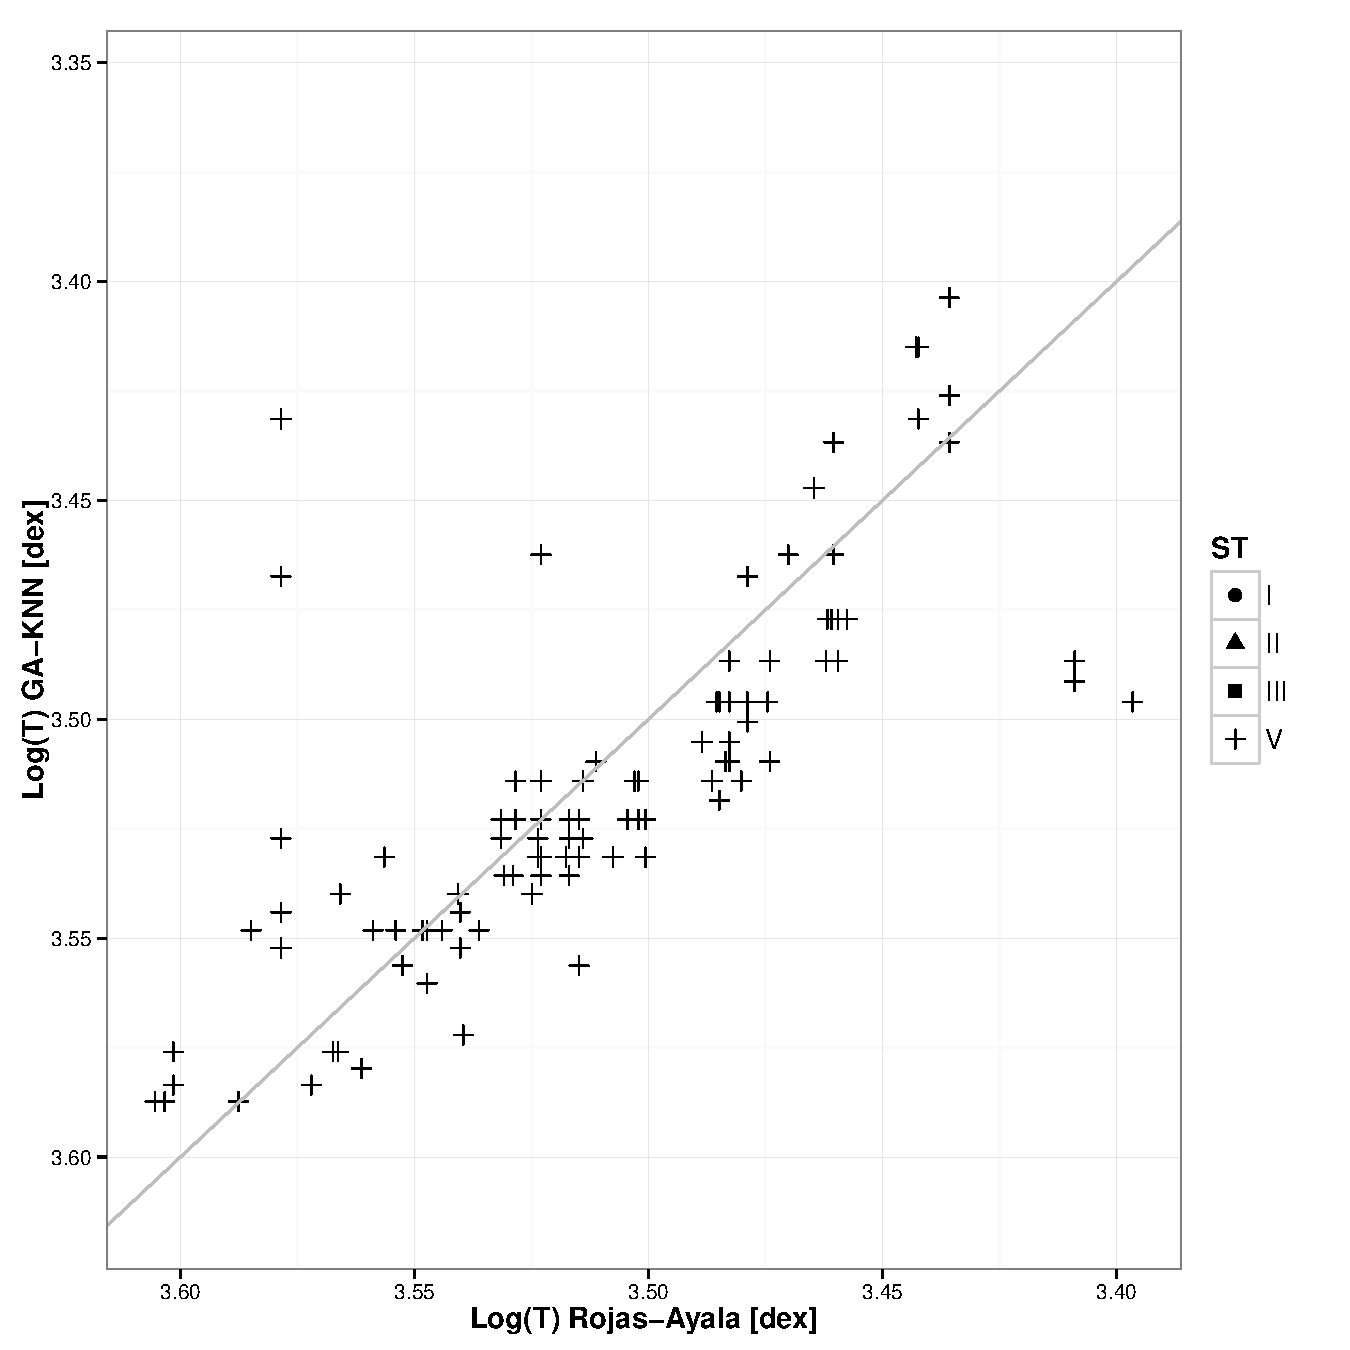
\includegraphics[width=9cm]{figs/ipac_LG_Trojas_Tknn_10.pdf}
 \caption{Relationship between $log(T) from Rojas-Ayala $ in the x axis 
 and $log(T)$ as predicted by KNN with SNR=$10$}
 \label{fig:ipac_lt_lt}
 \end{center}
\end{figure}
%%%%%%%%%%%%%

\subsubsection{Surface gravity models}

As in the IRTF exercise, we attempt to select features for surface
gravity estimation from BT-Settl spectra using GAs despite the much
lower spectral resolution and smaller wavelength coverage of the IPAC
spectra. Since there is no substantive compilation of surface
gravities that we could cross match with the IPAC list of M stars in
the Dwarf Archive, we are left with the same plausibility arguments
used in the IRTF study which are based on the $\log(T_{\rm
  eff})$--$\log(g)$ diagram.

We again use the effective temperatures as input of the regression
models. Table~\ref{tab:models_G_rmse} shows the cross-validation RMSE
and RMDSE for the same set of regression models used throughout this
article. It shows that the GA-RF model outperforms all other in all
SNR regimes, giving a consistent RMDSE of 1.0 dex. Obviously, this is
barely enough for classification in luminosity classes.

% HERE 2: This must be wrong: the Chi^2 and ICA columns are almost empty
% so I have asked Joaquín why. If the RMDSE are computed from these empty columns, these figures are just wrong.
% Answer: Wrong RData
% REDO tables and discussion

\ra{1.3}
\begin{table*}\centering
\begin{tabular}{@{}rrrcrrcrr@{}}\toprule
& \multicolumn{2}{c}{$SNR = 10$} & \phantom{ab}& \multicolumn{2}{c}{$SNR = 50$} &
\phantom{ab} & \multicolumn{2}{c}{$SNR = \infty$}\\
\cmidrule{2-3} \cmidrule{5-6} \cmidrule{8-9}
$Regression Models$ & $RMSE$ & $RMDSE$ && $RMSE$ & $RMDSE$     && $RMSE$       & $RMDSE$ \\ \midrule
$\chi^2$    & 2.2       & 1.6       && 2.2       & 1.4       && 2.2       & 1.6 \\
PPR-ICA     & 2.1       & 1.8       && 1.8       & 1.4       && 4.3       & 4.2 \\
GA-RF       & {\bf 1.3} & {\bf 1.0} && {\bf 1.6} & {\bf 1.1} && {\bf 1.4} & {\bf 0.9} \\
GA-GBM      & 1.6       & 1.1       && 1.7       & 1.4       && 1.7       & 1.2 \\
GA-SVR      & 2.0       & 1.8       && 2.1       & 1.9       && 2.3       & 1.6 \\
GA-NNET     & 2.0       & 1.8       && 2.2       & 1.9       && 3.2       & 2.8 \\
GA-MARS     & 1.8       & 1.5       && 2.0       & 1.7       && 2.0       & 1.5 \\
GA-KNN      & 2.0       & 1.5       && 2.2       & 1.7       && 1.7       & 1.2 \\
GA-KPLS     & 1.8       & 1.4       && 2.0       & 1.7       && 2.7       & 2.3 \\
GA-RR       & 2.0       & 1.8       && 2.1       & 1.8       && 3.7       & 3.2 \\

\bottomrule
\end{tabular}
\caption {RMSE and RMDSE for the various regression models predicting $Log(G)$ [dex].} 
\label{tab:models_G_rmse} 
% \end{center}
\end{table*}

% THIS PARAGRAPGH NEEDS REWRITING
Figure \ref{fig:teffvsloggIPAC} shows the $\log(T_{\rm
  eff})$--$\log(g)$ diagram for the GA-RF and GA-NNET models. The
  latter is, in our opinion, the one that shows the diagram that is
  most with Fig. \ref{} in this work, and Fig. 1
  in \cite{cesetti}. All GA- models predict decreasing surface
  gravities for main sequence stars below $\log(T_{\rm
  eff}=3.6$. GA-NNET predicts main sequence values between
  $4 \le \log(g) \le6$, while luminosity classes III-I appear clearly
  separated from the main sequence with values concentrated in the 4-6
  range except for the hottest cases with $\log(T_{rm eff} >
  3.55$. The GA-RF results, despite showing the best cross-validation
  errors (RMSE/RMDSE), result in unrealistic main sequence
  gravities. We interpret this as the result of overfitting to the
  training examples.

\begin{figure*}
 \begin{center}
 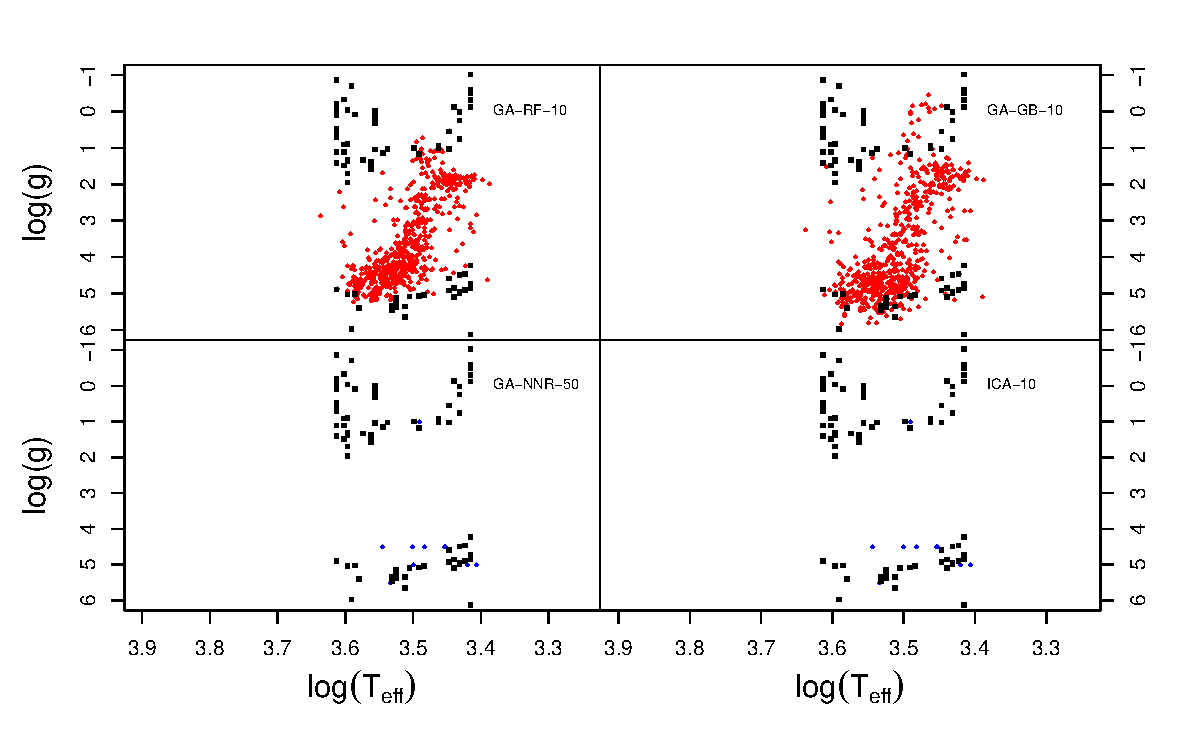
\includegraphics[width=\textwidth]{figs/ipac-teff-logg.pdf}
 \caption{Relationship between $log(T) $ ($x$ axis) 
 and $log(g)$ ($y$ axis) for several regression models.}
 \label{fig:teffvsloggIPAC}
 \end{center}
\end{figure*}

{\bf Right now, it appears that feature selected models are worse than
$\chi^2$, judging only from the 10 available estimates (mail sent to
jbmere). If so, the conclusion is clear: we should not do feature
selection at these resolutions. This is useful as Cesseti et al do not
question the utility of feature selection. For the IRTF (which is the
dataset used by Cesseti et al), we should check this: are the models
with feature selection better than $\chi^2$?}

\subsubsection{Metallicity models} 

Finally, the same analysis is performed for metalicities, again using
the previously inferred temperature as a fixed input feature.
Table~\ref{tab:models_M_rmse} shows a summary of the cross-validation
performance of the different models.

In general, models trained with SNR=$\infty$ show much poorer 
performace except for the GA-RF and GA-GBM cases. The best $\chi^2$ 
model produces errors almost a factor two larger than the 
$GA-RF-\infty$ model (although it has to be borne in mind that, while 
our regressors are capable of predicting metallicities that are 
intermediate in the grid, the minimum $\chi^2$ can only yield values 
in the grid, which has a step size of 0.5 dex). Models trained with 
SNR=10 and 50, on the contrary,  show a more consistent behaviour for 
the entire set of regressors, with poorer performances than the 
apparently optimal $GA-RF-\infty$, but also smaller differences between models. 

%
% Metalicidad teórica desde NevesIII para IPAC
%
% Check if this comes from CV if not, replace
\ra{1.3}
\begin{table*}\centering
\begin{tabular}{@{}rrrcrrcrr@{}}\toprule
& \multicolumn{2}{c}{$SNR = 10$} & \phantom{ab}& \multicolumn{2}{c}{$SNR = 50$} &
\phantom{ab} & \multicolumn{2}{c}{$SNR = \infty$}\\
\cmidrule{2-3} \cmidrule{5-6} \cmidrule{8-9}
$Regression Models$ & $RMSE$ & $RMDSE$ && $RMSE$ & $RMDSE$     && $RMSE$       & $RMDSE$ \\ \midrule
$\chi^2$    & 0.55 & 0.27 && 0.51 & 0.29 && 0.43  & 0.29 \\
$PPR-ICA$   & 0.48 & 0.27 && 0.70 & 0.39 && 0.85  & 0.71 \\
$GA-RF$     & 0.55 & 0.38 && 0.71 & 0.61 && 0.23  & 0.16 \\
$GA-GBM$    & 0.64 & 0.43 && 0.87 & 0.84 && 0.31  & 0.23 \\
$GA-SVR$    & 0.46 & 0.26 && 0.57 & 0.44 && 3.38  & 2.33 \\
$GA-NNET$   & 0.52 & 0.45 && 0.66 & 0.54 && 2.03  & 1.88 \\
$GA-KNN$    & 0.37 & 0.28 && 0.99 & 0.78 && 0.56  & 0.32 \\ 
$GA-MARS$   & 0.71 & 0.47 && 0.80 & 0.69 && 1.15  & 0.68 \\
%$ pls $    & 0.67  & 0.61  && 0.63  & 0.55 && 1.17 & 1.02 \\ 
$GA-RR$     & 0.47 & 0.29 && 0.50 & 0.36 && 1.18  & 1.18 \\

\bottomrule
\end{tabular}
\caption {RMSE and RMDSE for the various regression models predicting $Met$ [dex].} 
\label{tab:models_M_rmse} 
% \end{center}
\end{table*}

In order to select the best model, we again compare our model predictions with the 
reference catalogs used in Sect. \ref{sect:irtf-met}. We select, as best model the 
Random Forest trained with noiseless synthetic spectra, which renders the minimum 
RMSE (0.3 dex). Figure \ref{fig:ipac_mt} shows the comparison of our 
estimates with the reference catalogs, using the same symbols and colours as in 
Fig. \ref{MIRTF_ICA_10}.  

Our value of the RMSE contrasts with the differences between estimates for the 
same star in the literature. We obtain a mean difference of 0.1 dex {\bf TO BE COMPLETED ALSO FOR IRTF}


%% Check results from cesseti and add a plot with best prediction

% FIGURE WITH LITERATURE METALLICITIES
\begin{figure}
 \begin{center}
 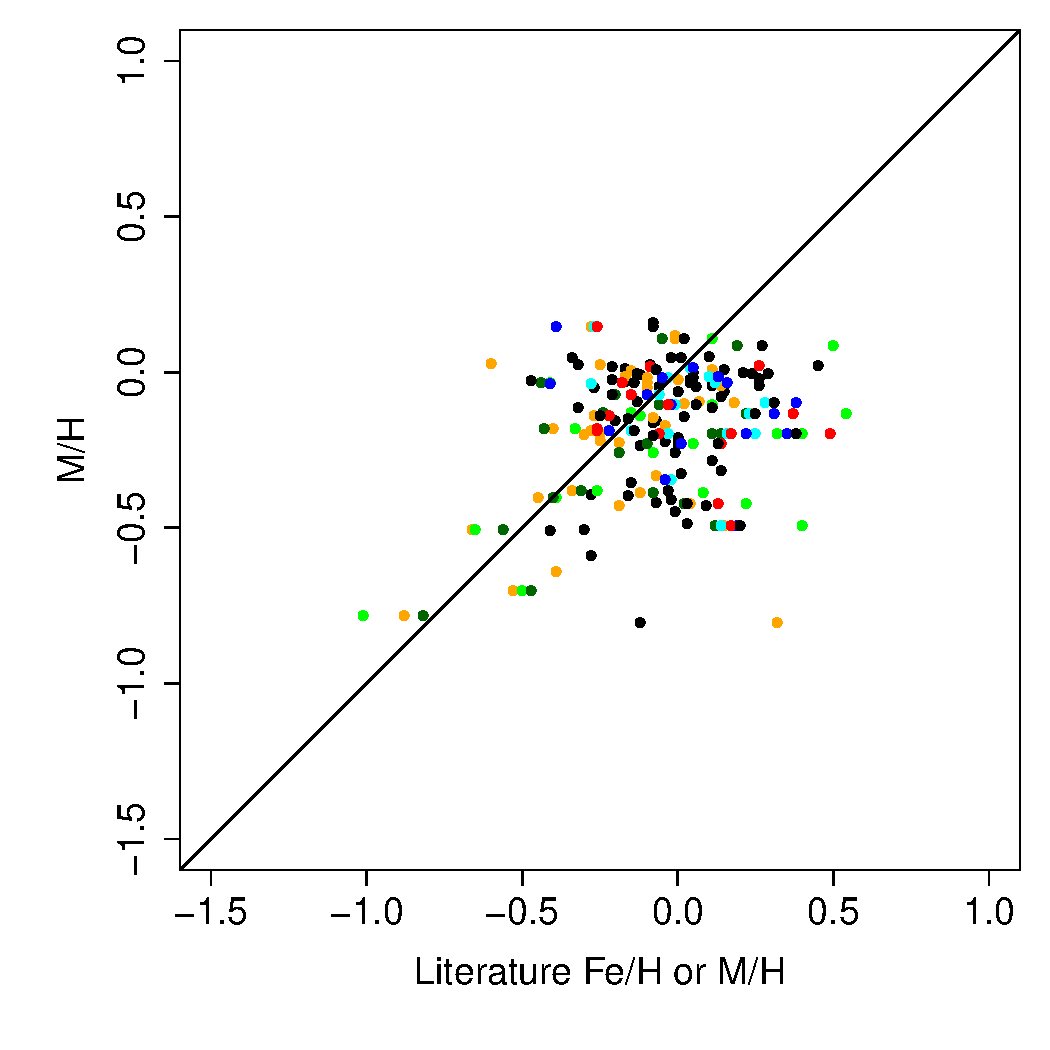
\includegraphics[width=9cm]{figs/ipac-figs/M-RFInf.pdf}
 \caption{Relationship between the $RF-\infty$ predictions for 
 	metallicity and values from the literature. 
 	Black empty circles represent values from \cite{cesetti}
 	; orange filled circles, values from \cite{NevesIII};  green filled 
 	squares, values that the Vizier catalog entry for Table 8 of 
 	\cite{NevesIII} links to \cite{Jao}, although we find no evidence that \cite{Jao} 
 	contains estimates of metallicities; cyan and blue filled squares, the values 
 	of [M/H] and [Fe/H] respectively in \cite{RA2012}; red filled squares, values 
 	from \cite{Mann2015}; yellow filled squares,  values from \cite{Newton2014}; and, 
 	finally, black filles squares, values from \cite{Gaidos2015}.}
 \label{fig:ipac_mt}
 \end{center}
\end{figure}


It is interesting to note that our predictions extend to metallicities as low as -2.1. Figure \ref{fig:ipac-hist-mets} shows a histogram of the metallicities predicted by the GA-RF-$\infty$ model for the IPAC set of spectra. We find predictions below -1.5 for eleven sources, 6 of which have been previously identified as subdwarfs of different categories (see Table \ref{tab:known-sds}).  

\begin{figure}
	\begin{center}
		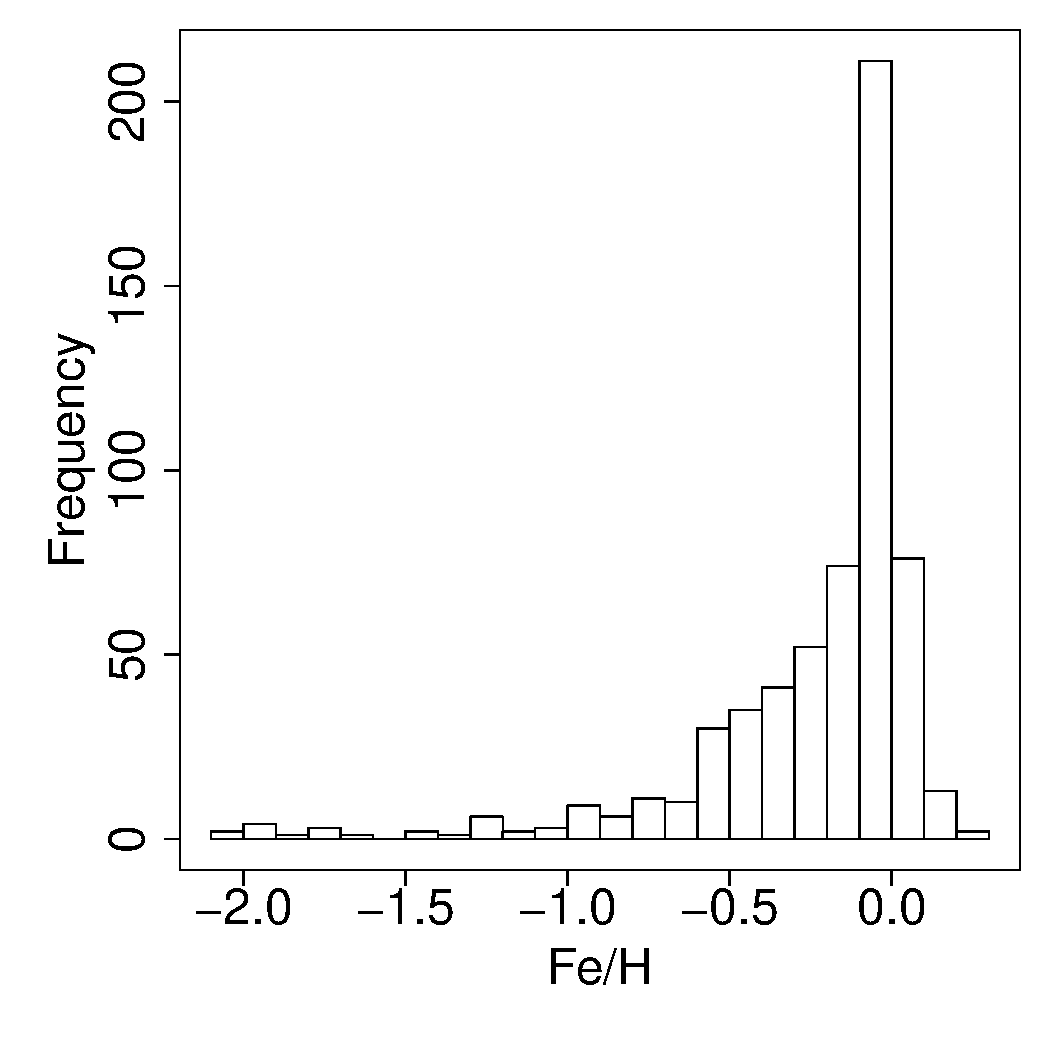
\includegraphics[width=9cm]{figs/ipac-figs/ipac-M-hist.pdf}
		\caption{}
		\label{fig:ipac-hist-mets}
	\end{center}
\end{figure}


\begin{table}\centering
	\begin{tabular}{@{}llll@{}}
		\toprule
		Identifier & classification & Reference & GA-RF-$\infty$\\
		\hline
		LHS 3768 & usdM3 & \cite{1995AJ....109..797K}  & -2.1 \\
		LHS 2352 & esd   & \cite{1995AJ....109..797K}  & -2.0 \\
		LHS 1691 & usdM2 & \cite{0004-637X-669-2-1235} & -1.95\\
		LHS 2023 & esdM6 & \cite{0004-637X-672-2-1153} & -1.95\\
		LHS 515  & esdM5 & \cite{1538-3873-117-833-676}& -1.8\\
		LP471-17 & sdM   & \cite{1995AJ....109..797K}  & -1.7\\
		\bottomrule
	\end{tabular}
	\caption{TMP TBC} 
	\label{tab:known-sds} 
\end{table}

The remaining 5 stars with metallicities below -1.5 are 2MASS J17275631-3240430 (-2.0 dex); 
LHS 1625 (-1.97 dex);  2MASS J19215188+2802275 (-1.9 dex); 2MASS J19004675+2806462 (-1.7 dex), 
classified as K7III by \cite{1994ApJS...94..749K}); and 2MASS J14465233-5320580 (-1.7 dex). 

